%~ \chapter{Results \& Improvements}   % former
\chapter{Results, Improvements \& Discussion}
\label{chap:results}

First we describe what tools we needed to perform a practical attack, then we present our results and discuss possible enhancements of the attack. Finally we outline why this attack is useful during white-box cipher design.

\section{Attack Tools}
\label{sec:tools}

Since there is no open-source toolkit\footnote{At the time of writing. However, it should be available soon from the original authors.} for the purpose of DCA described in Section \ref{sec:scawbc}, we implemented it ourselves. Our toolkit consists of several tools and subtools, see the following list.

%!% vočekovat, Teuwen psal mail že to brzy uvolní jako open-source

\begin{itemize}
	\item Acquire traces (see Section \ref{sec:tracq}):
	\begin{itemize}
		\item acquire single trace (PIN tools, modified versions of Teuwen's one \cite{teuwen2015movfuscator}),
		\begin{itemize}
			\item memory reads/writes and their addresses/contents,
		\end{itemize}
		\item manage trace acquisition (generate \& save respective plaintexts along).
	\end{itemize}
	\item Filter traces (see Section \ref{sec:filter}):
	\begin{itemize}
		\item filter constant entries \& save its mask $M_C$ (see Figure \ref{fig:constmask}),
		\item filter by address and temporal range,
		\begin{itemize}
			\item acquire another {\em full} trace $T$ (preferably in the same terminal session),
			\item filter it with mask $M_C$ yielding $T_C$,
			\item visualize $T_C$,
			\item estimate address \& temporal range,
			\item create another mask $M_R$ based on the range using $T_C$,
			\item filter all traces with $M_R$ (see Remark \ref{rem:rangemask}).
		\end{itemize}
	\end{itemize}
	\item Attack traces (see Section \ref{sec:attack}):
	\begin{itemize}
		\item run attack,
		\begin{itemize}
			\item CPA attack (Algorithm \ref{alg:cpa}), or
			\item bit-wise DPA attack (Algorithm \ref{alg:bitwisedpa}),
		\end{itemize}
		\item process \& display results.
	\end{itemize}
\end{itemize}


\section{Results}
\label{sec:results}

First we used our toolkit to attack our straightforward implementation of AES, here named {\tt naiveAES}, which served just as a proof-of-concept. Then we performed the most interesting attack which Bos et al. \cite{bos2015differential} did -- we successfuly attacked Klinec's implementation \cite{klinec2013implementation} of WBAES by Chow et al. \cite{chow2003aes}, here named {\tt KlinecWBAES}.

Note that the following Section \ref{sec:naiveaes} giving results of attack against {\tt naiveAES} does not fully cover many details, these are given separately in the subsequent Section \ref{sec:klinecwbaes} with results of attack against {\tt KlinecWBAES}.


% ======================================================================
% ===   n a i v e A E S                                              ===
% ======================================================================

\subsection{\tt naiveAES}
\label{sec:naiveaes}

In order to prove the concept of both SCA algorithms presented in this thesis, we first attacked our straightforward AES implementation {\tt naiveAES} with both of them.

\subsubsection{CPA against {\tt naiveAES}}
	
	We repeated CPA attack (i.e. Algorithm \ref{alg:cpa}) with $10$ different keys and for different amounts of plaintexts. See results in Table \ref{tab:naiveaes}.
	
	\begin{table}[H]
		\begin{center}
		\begin{tabular}{| c | c | c | c |}
			\hline
			~ & \multicolumn{2}{c|}{\bf $n\times n$ squares} & {\bf Computational} \\
			~ & \multicolumn{1}{c}{Lower bound} & \multicolumn{1}{c|}{Upper bound} & {\bf Power}\\
			\hline
			2D & \multicolumn{2}{c|}{See see} & Universal \\
			\hline
			2D & see & see & Unknown \\
			\hline
		\end{tabular}
		\end{center}
	\caption{CPA against }
	\label{tab:naiveaes}
	\end{table}

\subsubsection{Bit-Wise DPA against {\tt naiveAES}}
	
	Algorithm \ref{alg:bitwisedpa}
	
	%?% vyzkoušet rijinv na naiveAES, nemělo by jít


% ======================================================================
% ===   K l i n e c W B A E S                                        ===
% ======================================================================

\subsection{\tt KlinecWBAES}
\label{sec:klinecwbaes}



%~ co jsem použil za implmentace, kolik traců, jak dlouho to běželo, že jsem zjistil adresu kde to leakuje
%~ teoreticky by mělo bejt popsáno v předch. kapitole, tady už bych jenom zmínil co jsem použil a co vypadlo
%~ a proč to s tou javou nešlo ... (ale vyzkoušet)
%~ de facto takovej protokol
%~ Two (?) implementations will be considered for the attack:
%~ \begin{itemize}
	%~ \item our naive AES implementation (C++), and
	%~ \item Klinec's implementation of White-Box AES \cite{klinec2013white} (C++).
%~ \end{itemize}
%~ NaiveAES implementation was broken by both algorithms, CPA attack required $x$ traces, bitwise DPA attack required $y$ traces.
%~ White-Box-AES implementation was only broken by bitwise DPA attack and many interesting things occured.
% provést útok s několikrát nagenerovanejma tabulkama (v manuálu pak popsat co je pro to potřeba udělat)



\section{Enhancements of the Attack}   %?% to/of ?
\label{sec:enhancements}

%~ Before we introduce our improvements, we present one of Bos et al.\ \cite{bos2015differential} and reproduce their results in order to have some comparison of our method with previous results.
In this section we propose our novel improvement of the attack and present its practical results. But before we do so, we introduce an enhancement by Bos et al.\ \cite{bos2015differential} and reproduce their results in order to have some comparison with previous results for our method.
%~ We will later use these reproduced results for comparison with our novel approach.
%~ We will later use these reproduced results as a reference for our novel approach.


% ==============================================================================
% ===   E X P L O I T I N G   W B A E S   S T R U C T U R E                  ===
% ==============================================================================

\subsection{Exploiting WBAES Structure}

WBAES by Chow et al.\ \cite{chow2002aes} has been shown by Klinec \cite{klinec2013white} to be eqivalent to Karroumi's improved version \cite{karroumi2011protecting}. Remind that Karroumi's WBAES uses internally dual AES'es and therefore we cannot recognize which affine mapping has been used inside SBoxes, see Note \ref{note:dualsbox}.

Let us first remind definition of the original SBox (Equation \ref{eq:sbox}) and also remind that the multiplication is not performed in $F$, but in the ring of binary polynomials instead:
\[
	\defsbox .
\]
Note that the original SBox is a specific affine mapping of Rijndael inverse of its input while in Karroumi's approach, this affine mapping is not fixed. Such a new SBox could be written as   %?% neni už to dopsaný tam dřív?
\begin{equation}
\label{eq:spq}
	S_{p,q}(A) = p\cdot A' + q \pmod{x^8+1}
\end{equation}
for $p,q\in F$ and $p$ coprime with $x^8+1$. The simplest affine mapping is obviously achieved for $p=1$ and $q=0$ which yields $S_{1,0}(A) = A'$ i.e.\ only a Rijndael inverse.

\begin{remark}
\label{rem:coprime}
	The reason why $p$ must be coprime with $x^8+1$ was already given in the definition of the original SBox in Note \ref{note:sboxinv} -- it was due to its invertibility. Hence we would like to test whether $p$ is coprime with $x^8+1$.
	
	Note that $x^8+1 = (x+1)^8$, therefore if $p$ is {\em not} coprime with $x^8+1$, then $1$ must be its root, and vice versa. This can be easily tested, indeed $p(1) = 0$ if the number of its terms is even. It follows that $p$ is coprime with $x^8+1$ if and only if the number of terms of $p$ is odd.
\end{remark}


% ==============================================================================
% ===   C H A N G I N G   A T T A C K   T A R G E T                          ===
% ==============================================================================

\subsection{Changing Attack Target}
\label{sec:rijinv}

Since all of these SBoxes are equivalent inside WBAES, Bos et al.\ came up with the idea of changing the target of the attack from the original SBox to its simplest variant -- Rijndael inverse.

\begin{remark}
\label{rem:spq}
	Technically we only substitute SBoxes on Line \ref{line:s0} and \ref{line:s1} of Algorithm \ref{alg:bitwisedpa} with their desired variant, hence yielding
	\begin{align}
	\begin{split}
	\label{eq:target}
		S_0 &\gets \Bigl\{ Traces[n] \Bigm| S_{1,0}\bigl(KGuess\xor PTs[n][i]\bigr)[j] = 0 \Bigr\} , \\
		S_1 &\gets \Bigl\{ Traces[n] \Bigm| S_{1,0}\bigl(KGuess\xor PTs[n][i]\bigr)[j] = 1 \Bigr\} .
	\end{split}
	\end{align}
	Remind that we always use precomputed SBox tables as already stated in Remark \ref{rem:attacklookup}.
\end{remark}

\begin{note}
\label{note:target}
	The term {\em target of the attack} or simply {\em target} will be used heavily in the following text, let us describe it a bit closer.
	
	Target is a function $T$ which inputs a key byte $K$ together with a respective plaintext byte $P$ and outputs a byte (for now) or a single bit (later), e.g.\ $T(K,P) = S_{1,0}(K\xor P)$ (cf.\ Equations \ref{eq:target}). Target bit is just a specific bit of target's output. According to the target bit, traces are split into the sets $S_0$ and $S_1$ in Algorithm \ref{alg:bitwisedpa}, respectively.
\end{note}

\subsubsection{Results using Rijndael Inverse}
	
	We conducted the same attack as in Section \ref{sec:klinecwbaes}, now with Rijndael inverse as the target (i.e.\ the simplest SBox variant), see results in Table \ref{tab:klinecrijinv}. Note that this is the second part of successfuly reproduced results of Bos et al.
	
	\afterpage{
		\clearpage   % To flush out all floats, might not be what you want
		\begin{landscape}
		\begin{table}[H]
			\begin{center}
			\begin{tabular}{| c | r@{.} l@{\quad}r | r@{.} l@{\quad}r | r@{.} l@{\quad}r | r@{.} l@{\quad}r | r@{.} l@{\quad}r | r@{.} l@{\quad}r | r@{.} l@{\quad}r | r@{.} l@{\quad}r |}
	\hline
	\multirow{2}{*}{Byte} & \multicolumn{24}{c|}{Target bits (percentual gap\quad rank)} \\
	\cline{2-25}
	~ & \multicolumn{3}{c|}{1. bit} & \multicolumn{3}{c|}{2. bit} & \multicolumn{3}{c|}{3. bit} & \multicolumn{3}{c|}{4. bit} & \multicolumn{3}{c|}{5. bit} & \multicolumn{3}{c|}{6. bit} & \multicolumn{3}{c|}{7. bit} & \multicolumn{3}{c|}{8. bit} \\
	\hline
	\hline
	1.&3&3&207&45&4&{$\blacksquare$}&9&4&4&7&4&252&2&6&253&11&0&252&43&6&{$\blacksquare$}&35&3&{$\blacksquare$}\\
	\hline
	2.&5&4&233&1&3&255&0&9&252&49&4&{$\blacksquare$}&4&1&216&8&6&255&10&6&255&47&9&{$\blacksquare$}\\
	\hline
	3.&0&5&254&9&5&209&20&6&{$\blacksquare$}&45&6&{$\blacksquare$}&7&0&254&0&4&225&8&9&247&2&8&189\\
	\hline
	4.&2&1&37&12&7&{$\blacksquare$}&10&7&251&2&0&{\weak$\blacksquare$}&7&2&{\weak$\blacksquare$}&4&9&252&0&7&231&9&0&242\\
	\hline
	5.&2&1&244&17&9&{$\blacksquare$}&5&7&250&0&4&231&2&5&134&2&0&79&5&8&214&3&6&223\\
	\hline
	6.&53&2&{$\blacksquare$}&1&3&253&8&9&255&9&0&254&38&2&{$\blacksquare$}&37&8&{$\blacksquare$}&43&6&{$\blacksquare$}&7&3&2\\
	\hline
	7.&24&5&{$\blacksquare$}&0&9&248&6&4&187&5&8&255&13&6&209&36&2&{$\blacksquare$}&0&9&184&2&7&227\\
	\hline
	8.&48&9&{$\blacksquare$}&7&4&255&4&2&255&6&5&242&8&1&234&1&9&253&47&2&{$\blacksquare$}&2&8&255\\
	\hline
	9.&0&3&227&0&6&156&6&0&237&2&5&243&14&4&229&6&2&232&51&3&{$\blacksquare$}&15&1&{$\blacksquare$}\\
	\hline
	10.&8&9&{\weak$\blacksquare$}&3&0&158&10&1&1&40&5&{$\blacksquare$}&4&2&253&12&2&{$\blacksquare$}&54&3&{$\blacksquare$}&50&1&{$\blacksquare$}\\
	\hline
	11.&4&7&248&51&7&{$\blacksquare$}&6&7&241&0&4&254&4&4&251&5&2&45&10&1&255&4&7&1\\
	\hline
	12.&43&2&{$\blacksquare$}&2&8&251&7&2&254&2&5&255&6&9&236&3&2&255&49&2&{$\blacksquare$}&6&2&254\\
	\hline
	13.&7&3&205&6&2&4&9&2&191&6&6&30&63&7&{$\blacksquare$}&14&7&{$\blacksquare$}&7&5&240&0&8&255\\
	\hline
	14.&61&4&{$\blacksquare$}&4&9&231&1&7&246&54&4&{$\blacksquare$}&1&9&248&9&7&253&15&8&{$\blacksquare$}&46&2&{$\blacksquare$}\\
	\hline
	15.&0&7&221&2&0&250&4&7&1&2&0&{\weak$\blacksquare$}&8&0&223&31&3&{$\blacksquare$}&1&4&1&21&0&225\\
	\hline
	16.&4&0&255&57&7&{$\blacksquare$}&6&5&229&4&3&254&47&1&{$\blacksquare$}&9&5&255&8&2&254&1&7&253\\
	\hline
\end{tabular}   %!% obrátit pořadí sloupečků !!!
			\end{center}
		\caption{Bit-Wise DPA attack against {\tt KlinecWBAES} using $1024$ traces, Rijndael inverse taken as the target.}
		\label{tab:klinecrijinv}
		\end{table}
		\end{landscape}
	}
	
	On average, there are about $27\%$ of successful strong candidates and about $30\%$ of both weak and strong ones.
	
	In both cases (i.e.\ Table \ref{tab:klinecsbox} and \ref{tab:klinecrijinv}), there are, for each key byte, usually either only few target bits which actually leak, or nothing leaks at all (e.g.\ \nth{9} byte in Table \ref{tab:klinecsbox} cannot be considered as leaking, since the gap is very small at \nth{7} bit and at \nth{8} bit, the gap is much larger for an incorrect candidate; this happens much more often if less traces are used).
	
	The most substantial practical benefit of attacking different targets is that those key bytes, which did not leak with one target, may possibly leak with another, cf. \nth{9} byte in both tables.


% ==============================================================================
% ===   C O N S I D E R I N G   A N O T H E R   T A R G E T S                ===
% ==============================================================================

\subsection{Considering Another Targets}
\label{sec:16targets}

The benefit of having higher chance of breaking the key led us to the idea of using yet another invertible affine mappings inside SBoxes (see Equation \ref{eq:spq}) besides the one of the original SBox and identity (i.e.\ those used by Bos et al.).

There seems to be plenty of them: number of $p$'s is equal to the number of binary polynomials with degree smaller than $8$ which are coprime with $x^8+1$, there are $128$ of them (follows from Remark \ref{rem:coprime}). Number of $q$'s is simply $256$, hence altogether there are $128\cdot 256 = 32\,768$ invertible affine mappings which could be used inside SBoxes to create another targets.

\newpage   %!% zmrd bez toho píčuje

\begin{remark}
\label{rem:pqeffect}
	We realized that there are certain classes of mappings which give very the same results.
	\begin{description}
		\item[Effect of $q$'s.]
			First let us see what happens if we change one bit of $q$ (here considered as a byte). It obviously only changes the output of our SBox at the same bit, finally yielding a swap of $S_0$ and $S_1$ in the attack algorithm (only at this target bit, of course). Note that this swap has no effect on results, since we are only interested in absolute difference of means of values inside $S_0$ and $S_1$. Hence we will consider $q = 0$, our SBoxes will then be linear mappings of Rijndael inverse.
		
		\item[Effect of $p$'s.]
			Second let us study the effect of different $p$'s. Note that $x$ is coprime with $x^8+1$ and $p$ is supposed to be coprime, too, therefore if we multiply $p$ by $x\pmod{x^8+1}$, the result is still coprime with $x^8+1$.
			
			Now let us see what multiplying by $x\pmod{x^8+1}$ actually does. If the result does not need to be reduced, it simply shifts coefficients of $p$ by one, e.g.\ $(x^4 + x + 1) \cdot x = x^5 + x^2 + x$. If it reaches $x^8$, e.g.\ $(x^7 + x^4 + x^3) \cdot x \pmod{x^8+1} = x^5 + x^4 + 1$, we get $1$ at the end so the shift is actually a cyclical shift.
			
			Remind that polynomials, which are coprime with $x^8+1$, have odd number of terms (see Remark \ref{rem:coprime}), hence repeating multiplication by $x$ yields $8$ distinct polynomials which we put in single equivalence class. Since there are $128$ coprime polynomials, we get $128/8=16$ such classes, see Table \ref{tab:classrepre} for representants of each class. Note that the effect is the same on bits representing polynomials.
			
			Since we assumed $q = 0$, the actual output of two SBoxes using $p$'s from single class is thus also only a cyclical shift of each other. It follows that the effect on results is only a cyclical shift of the results among target bits. Hence also the information which target bit leaks is totally irrelevant.
	%?% neni zas tak irelevant ptž z pozice v trace zjistim která varianta to je, ze všech mi to pak může něco prozradit
	% => je irrelevant ptž ikdyž leaknou dva tak rozhodně nejsou od sebe jak by měly
	\end{description}
\end{remark}

\begin{table}[h]
	\begin{center}
	\begin{tabular}{| c | c | c | c | c | c | c | c |}
		\hline
		{\tt 01} & {\tt 07} & {\tt 0b} & {\tt 0d} & {\tt 13} & {\tt 15} & {\tt 19} & {\tt 1f} \\
		\hline
		{\tt 25} & {\tt 2f} & {\tt 37} & {\tt 3b} & {\tt 3d} & {\tt 57} & {\tt 5b} & {\tt 7f} \\
		\hline
	\end{tabular}
	\end{center}
\caption{Representants of classes of $p$'s in hexadecimal form. Remind that $p$ of the original SBox is {\tt 1f}.}
\label{tab:classrepre}
\end{table}

It follows that we can narrow down our attention to $16$ targets only. Indeed, our targets will be of the form $T(K,P) = S_{p,0}(K\xor P)$ for all representants $p$, see Table \ref{tab:classrepre}. Remind that Bos et al.\ only used the original SBox (i.e.\ $p = \texttt{1f}$) and Rijndael inverse (i.e.\ $p = \texttt{01}$).


% ==============================================================================
% ===   A T T A C K   U S I N G   A L L   1 6   T A R G E T S                ===
% ==============================================================================

\subsection{Attack Using All 16 Targets}

We attacked {\tt KlinecWBAES} using all of the $16$ attack targets and $1024$ traces, see results of the \nth{1} byte in Table \ref{tab:lintargets}. Note that the row of target {\tt 01} is indeed equal to the row of the \nth{1} byte in Table \ref{tab:klinecrijinv} and the row of target {\tt 1f} is indeed equal to the row of the \nth{1} byte in Table \ref{tab:klinecsbox}. Also note that the target {\tt 25} does not unravel the \nth{1} key byte even with $1024$ traces -- here we can clearly see the benefit of having many targets.

\afterpage{
	\clearpage   % To flush out all floats, might not be what you want
	\begin{landscape}
	\begin{table}[H]
		\begin{center}
		\begin{tabular}{| c | l@{\;} r@{.}l | l@{\;} r@{.}l | l@{\;} r@{.}l | l@{\;} r@{.}l | l@{\;} r@{.}l | l@{\;} r@{.}l | l@{\;} r@{.}l | l@{\;} r@{.}l |}
	\hline
	Tg. & \multicolumn{24}{c|}{Target bits} \\
	\hline
	{\tt 01}&\quad&0&15&$\square$&17&72&\quad&6&93&\quad&4&65&\quad&5&37&\quad&1&07&$\square$&13&48&$\blacksquare$&25&72\\
	\hline
	{\tt 07}&\quad&5&24&\quad&8&67&\quad&4&06&$\blacksquare$&47&88&\quad&8&15&$\square$&25&40&\quad&0&32&\quad&3&87\\
	\hline
	{\tt 0b}&$\square$&0&16&\quad&2&73&\quad&0&19&\quad&1&60&\quad&0&28&\quad&4&03&$\square$&18&07&$\blacksquare$&45&42\\
	\hline
	{\tt 0d}&$\blacksquare$&42&69&\quad&8&39&\quad&2&55&\quad&0&88&\quad&7&62&\quad&2&05&\quad&3&13&\quad&12&27\\
	\hline
	{\tt 13}&\quad&2&66&\quad&13&33&$\blacksquare$&28&97&\quad&2&38&\quad&2&56&$\square$&3&62&\quad&0&08&\quad&1&79\\
	\hline
	{\tt 15}&\quad&0&13&\quad&1&66&$\boxtimes$&13&94&\quad&4&78&\quad&0&94&\quad&6&47&\quad&0&22&$\square$&1&23\\
	\hline
	{\tt 19}&\quad&7&19&\quad&4&00&\quad&3&61&\quad&2&74&$\square$&7&60&$\boxtimes$&13&72&\quad&2&24&\quad&3&40\\
	\hline
	{\tt 1f}&$\square$&13&87&\quad&15&84&\quad&7&84&$\blacksquare$&38&56&\quad&0&84&\quad&3&72&\quad&3&59&\quad&6&76\\
	\hline
	{\tt 25}&\quad&5&15&\quad&0&84&\quad&0&48&\quad&1&19&$\boxtimes$&14&40&\quad&0&27&\quad&8&53&\quad&4&56\\
	\hline
	{\tt 2f}&$\blacksquare$&18&82&\quad&11&51&\quad&2&48&\quad&0&72&\quad&0&15&\quad&2&95&\quad&6&51&\quad&3&12\\
	\hline
	{\tt 37}&\quad&4&94&\quad&2&77&\quad&1&98&\quad&13&79&$\square$&4&98&\quad&0&66&$\boxtimes$&14&60&\quad&0&81\\
	\hline
	{\tt 3b}&\quad&0&46&$\blacksquare$&31&49&\quad&8&95&\quad&3&78&\quad&0&71&\quad&2&72&$\square$&0&32&$\square$&20&45\\
	\hline
	{\tt 3d}&\quad&6&83&\quad&0&93&\quad&3&67&$\boxtimes$&9&47&\quad&7&55&\quad&5&45&\quad&5&62&\quad&5&31\\
	\hline
	{\tt 57}&\quad&2&00&\quad&8&06&\quad&12&50&\quad&7&71&\quad&0&89&$\blacksquare$&15&48&\quad&2&39&\quad&2&37\\
	\hline
	{\tt 5b}&$\blacksquare$&25&00&\quad&2&07&$\square$&2&40&\quad&5&06&\quad&14&05&\quad&0&26&\quad&9&40&\quad&5&56\\
	\hline
	{\tt 7f}&\quad&4&63&\quad&4&79&\quad&6&66&\quad&1&48&\quad&0&20&$\blacksquare$&47&59&\quad&1&34&\quad&2&95\\
	\hline
\end{tabular}   % zašedit pod 10%
		\end{center}
	\caption{Bit-Wise DPA attack against {\tt KlinecWBAES} using $1024$ traces and all $16$ targets.}
	\label{tab:lintargets}
	\end{table}
	\end{landscape}
}


% ==============================================================================
% ===   N O N - I N V E R T I B L E   A F F I N E   M A P P I N G S          ===
% ==============================================================================

\subsection{Non-Invertible Linear Mappings}
\label{sec:noninv}

Another surprising results emerged with the idea of trying to use also non-invertible linear mappings in the attack targets. Remind that the mappings were originally required to be invertible, otherwise the resulting cipher would not be invertible. But there is no such limitation on attack target -- the attack is actually only required to work, no matter why.

As before, we only kept one representant of each class where elements are a multiple of $x^i\pmod{x^8+1}$ of each other, for some $i$. See these representants in Table~\ref{tab:classreprenoninv}.

\begin{table}[h]
	\begin{center}
	\begin{tabular}{| c | c | c | c | c | c | c | c | c | c |}
		\hline
		{\tt 00} & {\tt 03} & {\tt 05} & {\tt 09} & {\tt 0f} & {\tt 11} & {\tt 17} & {\tt 1b} & {\tt 1d} & {\tt 27} \\
		\hline
		{\tt 2b} & {\tt 2d} & {\tt 33} & {\tt 35} & {\tt 3f} & {\tt 55} & {\tt 5f} & {\tt 6f} & {\tt 77} & {\tt ff} \\
		\hline
	\end{tabular}
	\end{center}
\caption{Representants of classes of non-invertible $p$'s in hexadecimal form.}
\label{tab:classreprenoninv}
\end{table}

We can immediately discard {\tt 00}, because it only gives $0$ (everything would fall into $S_0$ in the attack algorithm). Also note that some classes include less than $8$ polynomials, e.g.\ $\texttt{11} = x^4+1$. This is because $(x^4+1)\cdot x^4 \pmod{x^8+1} = x^4+1$. For this reason, some target bits are not shown in results since their values would be repeating. You can find results of attack against {\tt KlinecWBAES} using $1024$ traces in Table~\ref{tab:noninvtargets}.

\afterpage{
	\clearpage   % To flush out all floats, might not be what you want
	\begin{landscape}
	\begin{table}[H]
		\begin{center}
		\begin{tabular}{| c | r@{.} l@{\quad}r | r@{.} l@{\quad}r | r@{.} l@{\quad}r | r@{.} l@{\quad}r | r@{.} l@{\quad}r | r@{.} l@{\quad}r | r@{.} l@{\quad}r | r@{.} l@{\quad}r |}
	\hline
	Target & \multicolumn{24}{c|}{Target bits (percentual gap\quad rank)} \\
	\hline
	\hline
	\multicolumn{25}{|c|}{\nth{0} byte} \\
	\hline
	{\tt 03}&33&4&$\blacksquare$&4&0&55&3&1&90&53&2&$\blacksquare$&5&0&149&4&5&207&4&2&224&20&4&$\blacksquare$\\
	\hline
	{\tt 05}&3&3&207&45&4&$\blacksquare$&9&4&4&7&4&252&2&6&253&11&0&252&43&6&$\blacksquare$&35&3&$\blacksquare$\\
	\hline
	{\tt 09}&9&2&255&4&0&172&12&2&207&55&8&$\blacksquare$&44&3&$\blacksquare$&10&1&232&2&0&190&7&6&84\\
	\hline
	{\tt 0f}&3&2&253&34&1&$\blacksquare$&4&7&224&3&1&238&0&9&207&7&2&212&0&9&232&0&6&238\\
	\hline
	{\tt 11}&5&5&17&1&9&240&5&7&206&2&2&186&\multicolumn{3}{c|}{---}&\multicolumn{3}{c|}{---}&\multicolumn{3}{c|}{---}&\multicolumn{3}{c|}{---}\\
	\hline
	{\tt 17}&14&8&$\blacksquare$&33&7&$\blacksquare$&2&9&233&1&4&252&2&0&236&2&0&226&3&8&$\blacksquare$&6&2&246\\
	\hline
	{\tt 1b}&3&6&63&41&0&$\blacksquare$&26&4&$\blacksquare$&26&0&251&14&1&$\blacksquare$&1&0&255&58&1&$\blacksquare$&6&6&155\\
	\hline
	{\tt 1d}&28&1&$\blacksquare$&52&9&$\blacksquare$&38&0&$\blacksquare$&34&9&$\blacksquare$&60&8&$\blacksquare$&3&2&253&5&0&157&51&1&$\blacksquare$\\
	\hline
	{\tt 27}&0&8&1&4&7&247&11&1&247&1&2&217&9&1&229&10&8&242&56&4&$\blacksquare$&1&4&104\\
	\hline
	{\tt 2b}&5&9&245&4&9&$\blacksquare$&4&7&250&48&4&$\blacksquare$&3&1&222&0&1&246&56&2&$\blacksquare$&8&4&247\\
	\hline
	{\tt 2d}&0&5&221&0&1&196&49&3&$\blacksquare$&1&3&239&18&7&$\blacksquare$&4&8&196&0&7&245&7&8&$\blacksquare$\\
	\hline
	{\tt 33}&0&2&221&11&7&$\blacksquare$&10&9&$\blacksquare$&5&0&215&\multicolumn{3}{c|}{---}&\multicolumn{3}{c|}{---}&\multicolumn{3}{c|}{---}&\multicolumn{3}{c|}{---}\\
	\hline
	{\tt 35}&4&8&244&8&4&228&47&9&$\blacksquare$&13&7&211&2&6&250&2&0&115&24&5&$\blacksquare$&18&5&$\blacksquare$\\
	\hline
	{\tt 3f}&5&2&249&3&7&109&4&9&$\blacksquare$&1&9&76&2&3&222&3&1&254&4&3&189&6&3&250\\
	\hline
	{\tt 55}&9&8&220&2&0&239&\multicolumn{3}{c|}{---}&\multicolumn{3}{c|}{---}&\multicolumn{3}{c|}{---}&\multicolumn{3}{c|}{---}&\multicolumn{3}{c|}{---}&\multicolumn{3}{c|}{---}\\
	\hline
	{\tt 5f}&6&1&225&5&7&245&39&6&$\blacksquare$&2&4&251&0&8&252&4&4&3&0&6&231&4&7&237\\
	\hline
	{\tt 6f}&3&4&86&34&3&$\blacksquare$&1&3&243&1&7&234&24&1&$\blacksquare$&17&5&$\blacksquare$&0&2&218&0&4&244\\
	\hline
	{\tt 77}&43&7&$\blacksquare$&2&2&219&0&1&194&7&5&130&\multicolumn{3}{c|}{---}&\multicolumn{3}{c|}{---}&\multicolumn{3}{c|}{---}&\multicolumn{3}{c|}{---}\\
	\hline
	{\tt ff}&0&0&223&\multicolumn{3}{c|}{---}&\multicolumn{3}{c|}{---}&\multicolumn{3}{c|}{---}&\multicolumn{3}{c|}{---}&\multicolumn{3}{c|}{---}&\multicolumn{3}{c|}{---}&\multicolumn{3}{c|}{---}\\
	\hline
	%~ \hline
	%~ \vdots & \multicolumn{3}{c|}{\vdots} & \multicolumn{3}{c|}{\vdots} & \multicolumn{3}{c|}{\vdots} & \multicolumn{3}{c|}{\vdots} & \multicolumn{3}{c|}{\vdots} & \multicolumn{3}{c|}{\vdots} & \multicolumn{3}{c|}{\vdots} & \multicolumn{3}{c|}{\vdots} \\
	%~ \hline
	\hline
	\multicolumn{25}{|c|}{\nth{3} byte} \\
	\hline
	\vdots & \multicolumn{3}{c|}{\vdots} & \multicolumn{3}{c|}{\vdots} & \multicolumn{3}{c|}{\vdots} & \multicolumn{3}{c|}{\vdots} & \multicolumn{3}{c|}{\vdots} & \multicolumn{3}{c|}{\vdots} & \multicolumn{3}{c|}{\vdots} & \multicolumn{3}{c|}{\vdots} \\
	\hline
	{\tt ff}&43&0&$\blacksquare$&\multicolumn{3}{c|}{---}&\multicolumn{3}{c|}{---}&\multicolumn{3}{c|}{---}&\multicolumn{3}{c|}{---}&\multicolumn{3}{c|}{---}&\multicolumn{3}{c|}{---}&\multicolumn{3}{c|}{---}\\
	\hline
	%~ \hline
	%~ \vdots & \multicolumn{3}{c|}{\vdots} & \multicolumn{3}{c|}{\vdots} & \multicolumn{3}{c|}{\vdots} & \multicolumn{3}{c|}{\vdots} & \multicolumn{3}{c|}{\vdots} & \multicolumn{3}{c|}{\vdots} & \multicolumn{3}{c|}{\vdots} & \multicolumn{3}{c|}{\vdots} \\
	%~ \hline
\end{tabular}
		\end{center}
	\caption{Bit-Wise DPA attack against {\tt KlinecWBAES} using $1024$ traces and non-invertible targets.}
	\label{tab:noninvtargets}
	\end{table}
	\end{landscape}
}


% ==============================================================================
% ===   L I N E A R   M A P P I N G S   O V E R   G F ( 2 )                  ===
% ==============================================================================

%~ \subsection{Considering Linear Mappings on $\GF(2)^8$ Over $\GF(2)$}
\subsection{Unifying Approach Considering $\GF(2)^8$ over $\GF(2)$}
\label{sec:unify}

Let us have a closer look at our previously considered targets, in particular at matrix representation of their internal linear mappings -- multiplication by $p\mod{x^8+1}$ (quick reminder: $T(K,P) = S_{p,0}(K\xor P) = p \cdot (K\xor P)' \mod{x^8+1}$). For now we will consider the linear mapping in the vector space $\GF(2)^8$ over $\GF(2)$, denoted by $\cal B$.

Note that equivalents of previously used linear mappings form a specific subset of all linear mappings on $\cal B$ since there are only $256$ of $p$'s. But there are obviously many more linear mappings on $\cal B$. Let us see how our previously considered mappings can be expressed -- they correspond with matrices with cyclically shifted rows as outlined in the following example.

\newpage   %!%

\begin{example}[Multiplication by $\texttt{3d}\pmod{x^8+1}$]
\label{ex:shiftmatrix}
	~ \\
	{\tt 3d} can be rewritten as $\texttt{3d} = x^5+x^4+x^3+x^2+1 \sim 00111101$, let further $A = a_7x^7+\ldots+a_1x+a_0$. Then we have
	\begin{align*}
		\texttt{3d} \cdot A \mod{x^8+1} &= (x^5+x^4+x^3+x^2+1) \cdot (a_7x^7+\ldots+a_1x+a_0) \mod{x^8+1} = \\
		&= (a_7+a_5+a_4+a_3+a_2)\cdot x^7 + ~\\
		&\quad\vdots \\
		&\quad + (a_7+a_6+a_5+a_4+a_1)\cdot x + ~\\
		&\quad + (a_6+a_5+a_4+a_3+a_0)\cdot 1 \sim \\
		&\sim
		\begin{pmatrix}
			\boxed{10111100} \\
			01011110 \\
			00101111 \\
			10010111 \\
			11001011 \\
			11100101 \\
			11110010 \\
			01111001 \\
		\end{pmatrix}
		\cdot
		\begin{pmatrix}
			a_7 \\ \vdots \\ a_1 \\ a_0
		\end{pmatrix} ,
	\end{align*}
	where {\tt 3d} can be found in reverse order in the first row of the corresponding matrix.
\end{example}

One may wonder whether we could get yet another set of targets when using another linear mappings, but actually we do not. Indeed, let us take a matrix $\mathbb{A}$ of an arbitrary linear mapping and observe the $j$-th bit of output (suppose that the $j$-th row of $\mathbb{A}$ is non-zero). Then this output bit is a scalar product of this row and the input.

Since the attack performs bit-wise, we would only care about the $j$-th row of $\mathbb{A}$. But note that there exists very the same row in some of our previously used linear mappings (now considered as a matrix over $\GF(2)$), let say on the $i$-th row of matrix $\mathbb{B}$. Indeed, we used all possible non-zero bytes and their equivalence classes were just inner cyclical shifts. So if we attack $i$-th target bit using $\mathbb{B}$, we obtain exactly the same results as with $j$-th target bit using $\mathbb{A}$.

It follows that we are actually only interested in non-zero vectors, there are $255$ of them. Note that there are indeed $255$ entries altogether in Table \ref{tab:klinecsbox} and \ref{tab:klinecrijinv}, for each byte.

The output of this kind of target is a scalar product of the non-zero vector and Rijndael inverse of input (cf.\ SBox construction in Equation \ref{eq:spq}), hence not a byte anymore, but a single bit (as already outlined in Note \ref{note:target}). Let us denote this mapping by
\begin{equation}
\label{eq:tba}
	T_B(A) = [B]^T\cdot [A'] ,
\end{equation}
where $B$ stands for the non-zero vector, $A'$ for Rijndael inverse of $A$, $[\cdot]$ for column vector representation and $[\cdot]^T$ for vector transposition, hence both vectors are scalar-multiplied. According to the notation of Note \ref{note:target}, it could be expressed as $T(K,P) = [B]^T\cdot [(K\xor P)']$.

This observation therefore does not bring any new targets, but a unifying and simplifying approach. Hence we do not give any results since these are already given in Table \ref{tab:lintargets} and \ref{tab:noninvtargets}.

We only wondered whether we should split our remarks in the following Section \ref{sec:remarks} by the origin of the linear mapping (i.e.\ either invertible, or non-invertible) and finally decided to do so, because there could possibly emerge some surprising results.

\subsubsection{Implementation Note}
	
	Now, as we have $255$ targets outputting only a single bit, we have to modify our attack (i.e.\ Algorithm \ref{alg:bitwisedpa}). We skip the forcycle on Line \ref{line:tbcycle} and alter also the following Line \ref{line:s0} and \ref{line:s1} into the following form:
	\begin{align*}
		S_0 &\gets \Bigl\{ Traces[n] \Bigm| T_B\bigl(KGuess\xor PTs[n][i]\bigr) = 0 \Bigr\} , \\
		S_1 &\gets \Bigl\{ Traces[n] \Bigm| T_B\bigl(KGuess\xor PTs[n][i]\bigr) = 1 \Bigr\} ,
	\end{align*}
	where $T_B$ is the mapping introduced in Equation \ref{eq:tba}. For this purpose we precompute all $255$ lookup tables for $T_B$'s, of course.
	


\section{Blind Attack}
\label{sec:blindattack}

In a real-world scenario, the key is typically unknown. Therefore we do not have any information whether our best candidate is correct or not. We need some rule to deduce so. Note that we can run ordinary AES encryption whenever we want to check our key candidate.

\begin{remark}
\label{rem:false}
	Especially note the attack against the \nth{1} byte using {\tt 3d} as a target and its last but one entry in Table \ref{tab:lintargets} -- here the incorrect candidate has a gap of almost $26\%$. It is actually the largest gap of an incorrect candidate among all targets and all bytes using this particular instance of WBAES tables. The largest gap of an incorrect candidate ever seen was almost $35\%$!
	
	In our results, the target bits keep their original order (but reverse), therefore we can deduce the row $B$ generating the target in terms of $T_B$. Here it is the second row of matrix of multiplication by $\texttt{3d}\pmod{x^8+1}$, see Example \ref{ex:shiftmatrix}. Hence the row is $B = 01011110$.
\end{remark}

For this reason, we studied our results deeper. The following section gives some of our remarks, next we suggest the blind attack itself in Section \ref{sec:subblindattack}


% ==============================================================================
% ===   R E M A R K S                                                        ===
% ==============================================================================

\subsection{Remarks}
\label{sec:remarks}

Obviously we cannot make conclusions based on single {\tt KlinecWBAES} table instantiation only. In order to avoid specific behavior of single instance, we created another $7$ instances, acquired $1024$ traces and ran attack against each key byte using all $255$ targets, for each instance. We processed the results and displayed several statistics. Here we present some of them. Note that we filtered correct candidates with a gap smaller than $10\%$ for this purpose.

\subsubsection{Leaking Bits}
	
	Remind that our trace is a bit-wise serialization of least significant bytes of memory addresses, hence we can identify which bit within that byte leaked -- simply by taking the leaking position within trace modulo $8$. This moduled position will be referred to as {\em leaking bit} (note the difference from target bit).
	
	We noticed soon that leaking bits are not very well balanced, therefore we put this data into a histogram, see Figure \ref{fig:leakbitall}. The histogram shows the amount of correct candidates with a gap larger than $10\%$ averaged over $8$ WBAES instances, for each leaking bit, together with standard deviation which is surprisingly very low. Note that the histogram does not provide absolute values since these could be misleading, only distribution is relevant at the moment.
	
	\begin{figure}[h]
	\begin{center}
		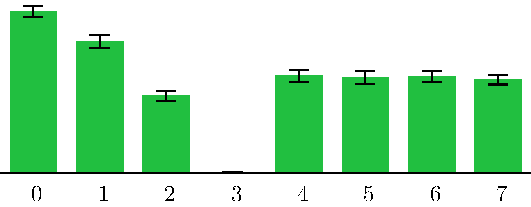
\includegraphics{figures/leak_bit/leak_bit.pdf}
		\caption{Average number of leaks and its standard deviation at each bit within trace.}
		\label{fig:leakbitall}
	\end{center}
	\end{figure}
	
	The \nth{0} and \nth{1} bits leaked slightly more, the \nth{2} bit slightly less and the \nth{3} bit actually leaked only twice while the overal average of the remaining bits was almost $160$! On the other hand, all of the remaining bits leaked fairly similarly. We do not have any explanation for this behavior.
	
	We further studied whether there is some influence of target invertibility (non-invertible targets were introduced in Section \ref{sec:noninv}).
	
	%!% že tam je furt kotel false positives, referovat, už jsem to zminoval v tom remarku myslim

\subsubsection{Leaks per Target}
	
	And now leaks per target. %!% remake: udělat všech nezávislejch 255 a počítat procentuelně (možností má 16, tak asi ne uplně histogram, ale spíš průměrnej počet leaků na target a nák otestovat uniformitu)
	% asi taky udělat víc útoků s různejma tabulkama ...
	%~ We repeated this attack against all key bytes using $1024$ traces and observed following:
	%~ \begin{itemize}
		%~ \item $12.6$ targets per byte were successful ($\blacksquare$) on average (without any limit on gap),
		%~ \begin{itemize}
			%~ \item the rest gave incorrect candidate ($\boxtimes$),
		%~ \end{itemize}
		%~ \item correct candidates had average gap of $37\%$ with standard deviation of $11\%$,
		%~ \item incorrect candidates had average gap of $13.5\%$ with standard deviation of $4.5\%$,
	%~ \end{itemize}
	%~ We used this information and repeated the attack with only $128$ traces while
	%~ \begin{itemize}
		%~ \item considering only candidates beyond $\mu_\textnormal{false}+3\sigma_\textnormal{false} = 27\%$, we get
		%~ \begin{itemize}
			%~ \item $10.6$ successful targets on average,
			%~ \item no false positive i.e.\ incorrect candidates are filtered out.
		%~ \end{itemize}
	%~ \end{itemize}
	
	\ldots will be changed. Makes no sense
	
	\begin{figure}[h]
	\begin{center}
		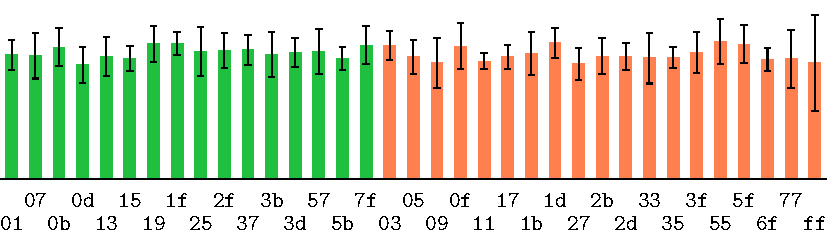
\includegraphics{figures/leak_target/leak_target.pdf}
		\caption{Success rate of each origin of target (previously denoted as $p$).}
		\label{fig:leaktargethist}
	\end{center}
	\end{figure}

\subsubsection{Using Less Traces}
	
	Note that once we use less traces, we usually do not find the correct candidate on the tail (as mentioned in Note \ref{note:tailrank}). Some results \ldots %!% results


% ==============================================================================
% ===   B L I N D   A T T A C K                                              ===
% ==============================================================================

\subsection{Blind Attack}
\label{sec:subblindattack}

\begin{note}
	This section only applies previous observations on a heuristic basis, there is no guarantee that our approach is the best.
\end{note}

We suggest to use less traces and repeat the attack with several targets. Even though we can hardly exploit the observation about candidates on the tail from Note \ref{note:tailrank}, it appears to be more robust and efficient to use several targets and sum the values of their respective best candidates unless filtered.

\ldots


% We rather suggest the following:
%~ \begin{enumerate}
	%~ \item pick a target, %!% Chi-square test of uniformity, pick random
	%~ \item attack using $256$ traces
%~ \end{enumerate}

%~ Therefore, in case of blind attack (i.e.\ no knowledge of actual key), we suggest to use less traces, but keep changing the target until the maximal gap exceeds $27\%$, then we accept that candidate. This is likely to happen soon since $10.6$ out of $16$ targets succeed on average.

% psal já / Teuwen:
%~ > I only wonder about the reasoning why Karroumi is more than Chow since
%~ > it seems to have been shown to be equal (based on what I wrote in my
%~ > previous email).
%~ 
%~ Well I've no problem to break completely Chow with standard DCA so there
%~ is something a bit more in Karroumi. Obviously not enough to make it
%~ robust enough...


\section{Use in White-Box Crypto Design}

Note that the attack allows us to reveal concrete physical addresses which contributed to the key recovery. Our intention was to find the corresponding piece of source code and later possibly also the value which is transformed into physical address -- it would most likely be an index in an array. We tried several approaches how to find that place in source code, see the following list.

\begin{description}
	\item[Watchpoint in GDB.]
		We set up a watchpoint in GDB running in the same terminal session while watching an address previously caught by PIN. Probably since PIN uses different environment, GDB did not catch the address at all.
		%!% zkusit valgrind a pak GDB?
	\item[GDB connected to PIN debugging interface.]
		We set up a connection between PIN application debugging interface and GDB as described in PIN manual \cite{pin214manual}, but could not catch {\em any} address. GDB was complaining that it cannot insert hardware breakpoint, on the other hand, software breakpoints did not work either.
		%!% vyzkoušet ten příklad z manuálu, jestli to jenom blbě nekompiluju ...
	\item[Outputting all array indexes.]
		Note that array indexes are very likely the values which are transformed to leaking physical addresses. Hence it should be possible to output and attack all indexes used within the encryption procedure. But, surprisingly, we did not succeed breaking the key from such ``traces''.
	%!% vyzkoušet debugger CLionu !!!
\end{description}

Each of these approaches appeared to bring valuable information about where the key leaks. The leakage position could be later used to identify a specific table access which leaks, hence it could possibly help us to clarify what is the actual reason why this attack works.

Note that, to the best of our knowledge, there is no explanation why this attack is actually possible. It seems impossible since all of the AES byproducts we attack are hidden by internal encodings, in fact random bijections. Note that a random bijection is extremely unlikely to provide any correlation between any input and output bit.

\ldots

% neni třeba problém v tom že to jsou concatenated encodings? i.e. ze 2x4 bitů postavený 8 bitový bijekce
% jesli takovejch už třeba neni moc málo nebo jestli náhodou nedávaj docela často nákou korelaci
% a ty skalární součiny neboli kousky lin. zobrazení jestli třeba nevylejzaj z input mixing bijection který jsou lin.
% třeba zkusit dokázat, že random bijection ani náhodou nezanechá korelaci v nákym bitu, mělo by tam bejt negligible
% asi se trochu rozepsat a odůvodnit ...
% třeba to, jak jsou ty bijekce generovaný, že to je z nákýho pejpru, kterej něco ukazuje
%~ The best known attack is BGE attack \cite{billet2005cryptanalysis} which is pure algebraic, on the other hand, this attack utilizes side-channel tools to attack memory traces instead.
Even though it is not fully understood, the benefit of this attack is obvious -- it introduces a principially different approach to break white-box crypto implementations. This attack may help to address weaknesses of a future white-box crypto implementation and possibly increase its resistancy to this kind of attack.

\subsection{Countermeasures against DCA}

\ldots

% proposed countermeasures against DCA?

